\chapter{Grundlagen und Stand der Technik}
\label{ch:basics}

Im folgenden werden zunächst die genutzten Frameworks und Tools erläutert, die zur Durchführung der Fallstudie benötigt wurden.
Dies sind neben Hadoop selbst auch die hierfür entwickelte, und in dieser Fallstudie genutzte, selbstadaptive Komponente für Hadoop, sowie die Plattform Hadoop"=Benchmark, die zur einfachen Ausführung eines Hadoop"=Clusters dient.
Zunächst wird jedoch das Framework \acrshort{ss} vorgestellt, das zur Durchführung der Fallstudie genutzt wurde.

%\section{Model Checking}\label{sec:modelchecking}

\ac{MC} ist eine Möglichkeit, um Systeme zu testen und zu verifizieren. Dazu werden vom \ac{MCr} alle möglichen Systemzustände in einem \emph{brute-force}-ähnlichem Vorgehen getestet und somit alle möglichen Szenarien getestet. Die Anzahl der Zustände kann sehr schnell $ 10^{120} $ oder mehr betragen \cite{Grumberg1999,Baier2008}.

\begin{figure}
	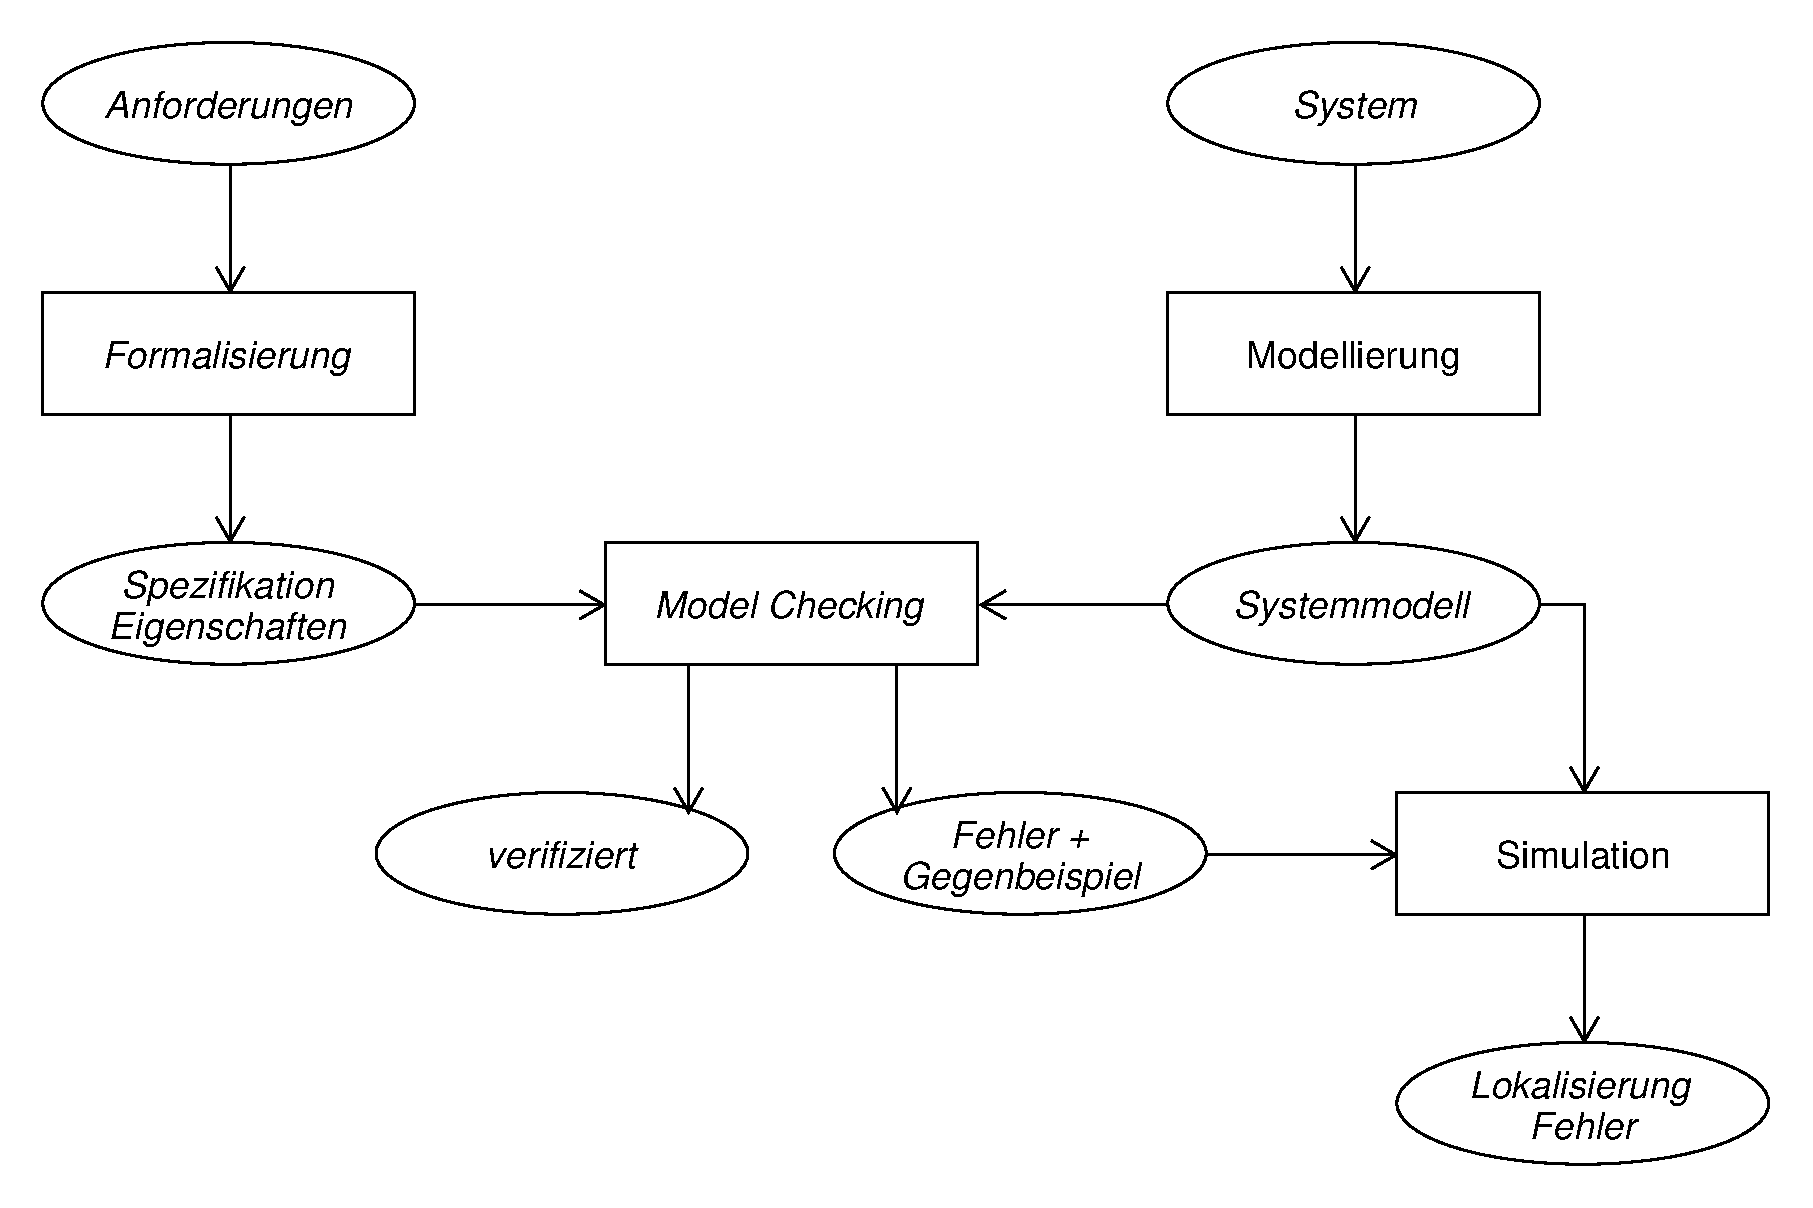
\includegraphics{./images/mcSchema.pdf}
	\caption[Schematischer Aufbau beim MC]{Schematischer Aufbau beim MC, nach \cite{Baier2008}}
	\label{fig:mcSchema}
\end{figure}

Ein \ac{MCr} nutzt, wie der Name schon sagt, ein Modell des Systems, um das System zu testen. Wie bei jeder anderen modellbasierten Technik ist daher die Qualität des \ac{MC} nur so gut wie das darauf zugrunde liegende Modell. Ein Modell kann auch als endlicher Automat angesehen werden, da ein Modell ebenfalls eine endliche Anzahl an möglichen Zuständen und dazugehörige Übergänge besitzt. Für jede Eigenschaft eines Zustandes muss zudem mithilfe einer sog. \emph{temporalen Logik}, also mathematisch bzw. formal, festgelegt werden, was gültige Werte dieser Eigenschaft sind. Die dazu benötigten Informationen werden aus den Anforderungen des Systems ermittelt und dem \ac{MCr} übergeben. So können später verschiedene Eigenschaften des gesamten Systems (\zB die formale Korrektheit, die Ausführbarkeit ohne Deadlocks oder die Einhaltung von Sicherheitsvorgaben) geprüft werden.

Zur Ausführung wird das gesamte Modell zunächst initialisiert und dann automatisch und systematisch vom \ac{MCr} auf Fehler und ungültige Zustände geprüft. In der Regel ist aber auch eine Ausführung als reine Simulation des Systems möglich, ohne explizit nach Fehlern zu suchen.

Wenn alle Zustände und deren Eigenschaften die Anforderungen erfüllen, erfüllt auch das Modell die Spezifikation. Wenn ein Zustand bzw. Eigenschaft die Anforderungen nicht erfüllt, prüft der \ac{MCr} anhand eines Gegenbeispiels den Ausführungspfad zum Fehler. Dadurch kann ermittelt werden, wo die Fehlerursache liegt. Einige der wesentlichen Fehlertypen und Ursachen sind:

\begin{description}
	\item[Modelling Error] Der Fehler liegt im Modell, welches korrigiert werden muss.
	\item[Design Error] Der Fehler liegt in den formellen oder informellen Anforderungen, dadurch muss das Modell und/oder die temporale Logik korrigiert werden.
	\item[Property Error] Der Fehler ist wirklich ein Fehler im System, welcher gefunden werden soll.
\end{description}

Möglich ist aber auch, dass die Ressourcen nicht ausreichen, um alle Zustände zu prüfen. In so einem Fall gibt es mehrere Möglichkeiten, damit umzugehen, \zB können Heuristiken oder Abstraktionen vom Modell genutzt werden \cite{Baier2008,Eberhardinger2016}.

\ac{MC} besitzt durch seine Charakteristik einige Vorteile, \uA \cite{Baier2008}:
\begin{itemize}
	\item \ac{MC} ist universell nutzbar, \zB für Software, Hardware oder eingebettete Systeme
	\item Partielle Verifikation ist möglich ohne das gesamte System testen zu müssen
	\item Vollständig automatisierbar und benötigt kaum Benutzerinteraktion oder hohe Expertise
\end{itemize}

Natürlich gibt es aber auch einige Nachteile, \uA \cite{Baier2008}:
\begin{itemize}
	\item Mit \ac{MC} wird nur ein Systemmodell und nicht das eigentliche System getestet, was weitere Fehler nicht ausschließt
	\item Hauptsächlich für steuerungsbasierte Anwendungen und nicht für datenbasierte Anwendungen geeignet
	\item Anzahl der möglichen Zustände kann zu hoch sein, um alle zu testen
\end{itemize}

Es gibt zahlreiche \ac{MC}-Frameworks, die bereits erwähnten \emph{LTSmin} und \emph{\sS} sind nur zwei davon.

\section{\acl{ss}}
\label{sec:ssharp}

\todo{Testen unter SS allgemein genauer erklären}
\textbf{\acf{ss}} ist ein am \isse der Universität Augsburg entwickeltes Framework zum Testen und Verifizieren von Systemen und Modellen.
Da es in \cS entwickelt wurde und \cS auch zum Entwickeln von Modellen und dazugehörigen Testszenarien genutzt wird, können zahlreiche Features des .NET"=Frameworks bzw. der Sprache \cS im Speziellen genutzt werden.
\ac{ss} vereint dabei die Simulation, die Visualisierung, modellbasierte Tests sowie die Verifizierung der Modelle durch einen \ac{MCr} \cite{Habermaier2015,Habermaier2016}.
Dadurch können alle Schritte einer vollständigen Analyse inkl. Modellierung direkt im Visual Studio ausgeführt werden und somit auch alle Features der IDE und .NET, wie \zB die Debugging"=Werkzeuge, genutzt werden.
Um entsprechende Analysen zu gewährleisten, hat das Framework jedoch auch einige Einschränkungen, wodurch \zB Schleifen und Rekursionen nur eingeschränkt bzw. nicht möglich sind.
Eine der größten Einschränkungen ist allerdings, dass während der Laufzeit keine neuen Objektinstanzen innerhalb des zu testenden Modells erzeugt werden können, sodass alle benötigten Instanzen bereits während der Initialisierung des Modells erzeugt werden müssen \cite{Habermaier2015}.

Um nun ein System testen zu können, muss dieses zunächst mithilfe von \cS-Klassen und -Instanzen modelliert werden.
Die dafür verwendeten Modelle sind meist stark vereinfacht und bilden nur die wesentlichen Aspekte der realen Systeme ab.
Für einen korrekten Test ist es jedoch wichtig, dass das Modell des Systems vergleichbar mit dem echten System ist.

Folgendes Beispiel zeigt den typischen, grundlegenden Aufbau einer \ac{ss}-Komponente:

\begin{lstlisting}[label=lst:ssExample,style=cs,
caption={Grundlegender Aufbau einer \acs{ss}-Komponente.}]
public class MyCOmponent : Component
{
  // fault definition, also possible: new PermanentFault()
  public readonly Fault MyFault = new TransientFault();
  
  // interaction logic (Fields, Properties, Methods...)
  
  // fault effect
  [FaultEffect(Fault = nameof(MyFault))]
  internal class MyFaultEffect : MyCOmponent
  {
    // fault effect logic
  }
}
\end{lstlisting}


Jede Komponente des Modells muss von \texttt{Component} erben, um als \ac{ss}-Komponente definiert zu sein.
Jede Komponente kann nun temporäre (\texttt{TransientFault}) oder dauerhafte (\texttt{PermanentFault}) Komponentenfehler enthalten, welche zunächst innerhalb der Komponente als Felder definiert werden. 
Der Effekt eines Komponentenfehlers wird anschließend in der entsprechenden Effekt"=Klasse definiert, welche von der Hauptklasse (hier \texttt{YarnNode}) erbt und mithilfe des Attributs \texttt{FaultEffectAttribute} dem dazugehörigen Komponentenfehler zugeordnet wird \cite{Habermaier2016}.

Um die Modelle zu testen, kommen in \ac{ss} verschiedene Werkzeuge zum Einsatz.
Eines davon ist eine reine Simulation, bei der das Framework nur einen Ausführungspfad ausführt und dabei keine Komponentenfehler aktiviert bzw. die Aktivierung \textit{manuell} gesteuert werden kann.
Ein weiterer Nutzen liegt in der Möglichkeit, im ausgeführten Ausführungspfad zeitliche Abläufe zu berücksichtigen, da hier das Modell Schritt für Schritt ausgeführt wird.
Hierbei wird für jede im Modell genutzte Komponente pro Schritt einmal die jeweilige Methode \texttt{Update()} aufgerufen, in der die jeweiligen Komponenten ihre Aktivitäten durchführen \cite{Habermaier2016}.

Ein anderes wichtiges Werkzeug von \ac{ss} ist die \ac{DCCA}, welche eine vollautomatische und \ac{MC}-basierte Sicherheitsanalyse ermöglicht.
Dabei wird selbstständig die Menge der aktivierten Komponentenfehler ermittelt, mit denen das Gesamtsystem nicht mehr rekonfiguriert werden kann und somit ausfällt.
Je nach Konfiguration können dazu auch Heuristiken genutzt werden, welche die Analyse beschleunigen und genauer machen können \cite{Eberhardinger2016}.
Dabei werden die verschiedenen aktivierten Komponentenfehler während der Analyse in tolerierbare und nicht-tolerierbare Fehler unterschieden.
Tolerierbare Komponentenfehler werden dazu genutzt, die Grenzen der Selbstkonfiguration des Systems zu ermitteln.
Dabei wird für jeden Systemzustand nach einer Rekonfiguration durch die \ac{DCCA} eine neue Fehlermenge ermittelt, mit der das System gerade noch lauffähig ist.
Das Auftreten eines tolerierbaren Komponentenfehler ist also gleichbedeutend mit einem einfachen Fehler im System, welcher die gesamte Funktionsweise des Systems nicht massiv einschränkt und eine Rekonfiguration noch ermöglicht.
Sobald jedoch ein Fehler auftritt, durch den eine Rekonfiguration des Systems nicht mehr möglich ist, wurde ein nicht-tolerierbarer Fehler gefunden, durch den das System nicht mehr funktionsfähig ist \cite{Habermaier2015}.

Das dritte Werkzeug zur Ausführung von Modellen in \ac{ss} ist der \ac{MCr} selbst.
Hierbei kann der in \ac{ss} bereits enthaltene, oder alternativ \emph{LTSmin}\footnote{\url{http://ltsmin.utwente.nl/}} genutzt werden \cite{SSWikiModelChecking}.
Beim \ac{MC} werden in einem \emph{brute-force}-ähnlichem Verfahren alle möglichen Zustände und Ausführungspfade in einem Modell mit einer endlichen Anzahl an Zuständen getestet.
Dadurch wird es ermöglicht, verschiedene Eigenschaften eines System zu testen und Fehler (\zB Deadlocks) zu erkennen \cite{Grumberg1999}.


\section{Apache Hadoop}
\label{sec:hadoop}

\textbf{Apache\texttrademark Hadoop\textregistered}\footnote{\url{https://hadoop.apache.org/}} ist ein Open"=Source"=Software"=Projekt, welches die Verarbeitung von großen Datenmengen auf einem verteilten System ermöglicht.
Hadoop wird von der \emph{Apache Foundation} entwickelt und stellt und enthält verschiedene vollständig skalierbare Komponenten.
Es ist daher möglich, ein Hadoop"=Cluster auf nur einem einzelnen PC, aber auch verteilt auf zahlreichen Servern auszuführen.
Hadoop ermöglicht es dadurch, sehr einfach Anwendungen auszuführen, um große Datenmengen zu verarbeiten.
Die für das Cluster, und damit den Anwendungen, verfügbaren Ressourcen beschränken sich lediglich auf die Summe der verfügbaren Ressourcen aller Hosts, auf denen das Cluster ausgeführt wird.

Hadoop besteht aus folgenden Kernmodulen \cite{HadoopHomePage}:

\begin{description}
	\item[Hadoop Common] \hfill \\
        Gemeinsam genutzte Kernkomponenten
	\item[Hadoop \acs{YARN} (\acl{YARN}\acused{YARN})] \hfill \\
        Framework zur Verteilung und Ausführung von Anwendungen und das dazugehörige Ressourcen"=Management
	\item[\acl{HDFS}] \hfill \\
        Kurz \acs{HDFS}\acused{HDFS}, verteiltes Dateisystem
	\item[Hadoop \acl{MR}] \hfill \\
        Kurz \acs{MR}\acused{MR}, Implementierung des \ac{MR}"=Ansatzes zum Verarbeiten von großen Datenmengen, nutzt \ac{YARN} zur Ausführung der Anwendungen
\end{description}

Aufgrund seiner Verbreitung stellt Hadoop eine der wichtigsten Implementierungen des \ac{MR}"=Ansatzes dar \cite{PoweredByHadoop}.
Die Eingabe"= und Ausgabedaten sind hierbei als \emph{Key"=Value}"=Paare definiert, die mithilfe des \ac{MR}"=Frameworks verarbeitet werden.
Hierbei werden zunächst die eingelesenen Eingabedaten in kleine und dadurch einfach zu verarbeitende Datenmengen aufgeteilt.
Die geteilten Daten werden dann in mehreren, parallel ausgeführten Map"=Tasks verarbeitet und zwischengespeichert.
Die zwischengespeicherten Daten werden anschließend von einem oder mehreren Reduce"=Tasks zusammengeführt und in die Ausgabedateien geschrieben.
Das Framework ist hierbei sehr Fehlertolerant, da ein fehlerhafter Task jederzeit neu gestartet werden kann \cite{Dean2004,Dean2010}.
Zur Speicherung der Ein-, Zwischen- und Ausgabedaten wird im Falle von Hadoop das \ac{HDFS} genutzt \cite{HadoopMapRedTutorial271}.
Für weitere Details zum \ac{MR}"=Framework sei hier auf \cite{Dean2004} und \cite{Dean2010} verwiesen, eine ausführliche Betrachtung des \ac{MR}"=Frameworks mit Vorteilen und Problemen lässt sich in \cite{Lee2012} finden.

Da das \ac{MR}"=Framework bzw. seine Implementierung in Hadoop nicht perfekt ist und in der Praxis zum Teil auch zweckentfremdet wurde, wurde in \cite{Vavilapalli2013} das \textbf{\ac{YARN}}"=Framework vorgestellt.
Die Kernidee ist hierbei die Trennung von Ressourcenmanagement und Scheduling vom eigentlichen Programm.
In diesem Kontext bildet der \ac{MR}"=Ansatz eine mögliche Anwendung, die mithilfe des \ac{YARN}"=Frameworks ausgeführt wird \cite{Vavilapalli2013}.

Ein Hadoop"=Cluster mit dem \ac{YARN}"=Framework besteht aus zwei wesentlichen Komponenten, dem \emph{Controller} mit \ac{RM} und den angeschlossenen \emph{Nodes}:

\begin{figure}[h]
    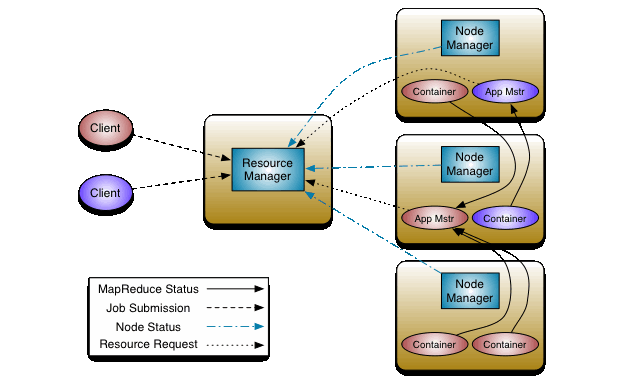
\includegraphics{./resources/yarn_architecture.png}
    \caption[Architektur des YARN"=Frameworks]
    {Architektur des \ac{YARN}"=Frameworks (entnommen aus \cite{HadoopYarnArch271})}
    \label{fig:yarnarch}
\end{figure}

Der \ac{RM} dient hierbei als \emph{Load"=Balancer} für das gesamte Cluster und besteht aus dem \ac{AM} und dem \emph{Scheduler}, die eigentliche Ausführung der Anwendungen findet auf den Nodes statt.
Der \ac{AM} ist für die Annahme und Ausführung von einzelnen Anwendungen zuständig, denen der Scheduler die dafür notwendigen Ressourcen im Cluster zuteilt.
Jeder Node besitzt einen \ac{NM}, der für die Überwachung der Ressourcen auf dem jeweiligen Node sowie der auf dem Node ausgeführten Anwendungs"=Container zuständig ist und diese Daten dem \ac{RM} übermittelt.

Jede \ac{YARN}"=Anwendung bzw. Job besteht aus einer oder mehreren Ausführungsinstanzen, genannt \emph{Attempts}.
Jeder Attempt besitzt einen eigenen \ac{AppMstr}, welcher das Monitoring der Anwendung und die Kommunikation mit dem \ac{RM} und \ac{NM} übernimmt und die dafür benötigten Informationen bereitstellt \cite{HadoopYarnArch271}.
Die eigentliche Ausführung einer Anwendung findet in den bereits erwähnten \emph{Containern} statt, die jeweils einem Attempt zugeordnet sind.
Container können auf einem beliebigen Node ausgeführt werden und repräsentieren die Ausführung eines Tasks innerhalb der Anwendung.

Zu erwähnen ist hier zudem, dass die Kommunikation zwischen den einzelnen Komponenten nicht in allen Fällen in Echtzeit statt findet.
Vor allem das Prüfen des generellen Node"=Zustandes durch den \ac{RM} wird bei einer Standard"=Konfiguration in periodischen Abständen von jeweils mehreren Minuten durchgeführt.
Sollte der \ac{NM} bei solchen Status"=Abfragen zunächst nicht reagieren, wird mehrere Minuten gewartet, bis der Node als defekt erkannt wird.
Ähnlich verhält es sich bei Zustandsabfragen an den \ac{AppMstr} \cite{HadoopYarnConfig271}.

Ein weiterer Bestandteil von Hadoop bzw. \ac{YARN} ist der \ac{TLS}.
Er ist speziell dafür entwickelt, die Metadaten und Logs der \ac{YARN}"=Anwendungen zu speichern und jederzeit, also als Anwendungshistorie, auszugeben \cite{HadoopYarnTlServer271}.

Zum Steuern des Clusters bzw. dem Monitoring der mithilfe von \ac{YARN} ausgeführten Anwendungen stellt Hadoop drei Schnittstellen zur Verfügung.
Dies sind eine graphische Weboberfläche, was zugleich auch die wichtigste Schnittstelle darstellt, entsprechende Befehle für die \acl{CLI} (engl. \emph{Command-line interface}, kurz \acs{CLI})\acused{CLI}, sowie eine REST"=API.
Während sich die Weboberfläche zur menschlichen Interaktion oder zum Finden von Fehlern eignet, dienen die \ac{CLI}"=Befehle vor allem zum Steuern des Clusters und die REST"=API zur automatisierten Rückgabe der Daten des Clusters zur Nutzung in anderen Programmen \cite{HadoopClusterSetup271,HadoopYarnCmds271,HadoopRmApi271,HadoopNmApi271}.

Das \textbf{\ac{HDFS}} basiert auf einer ähnlichen Architektur wie \ac{YARN} und besitzt ebenfalls einen Controller und mehrere Nodes:

\begin{figure}[h]
    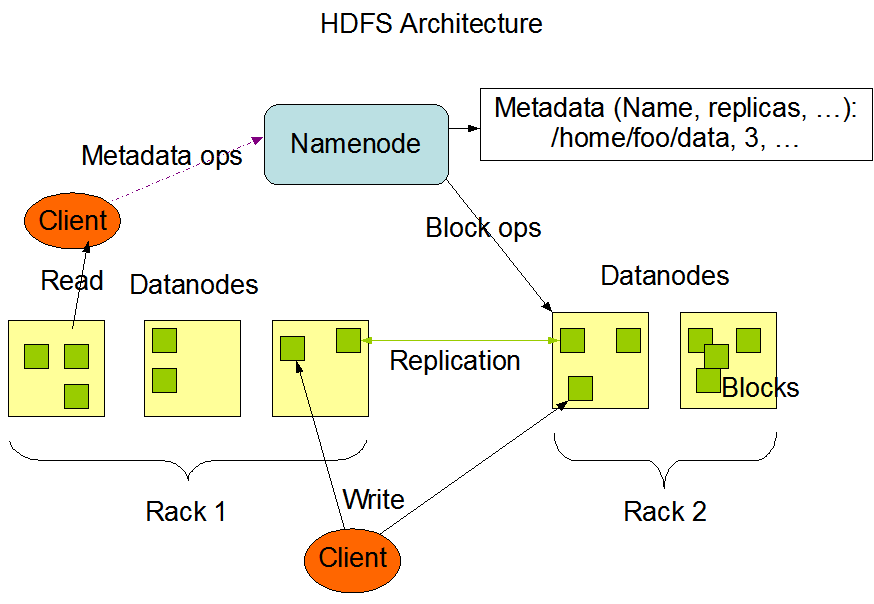
\includegraphics{./resources/hdfsarchitecture.png}
    \caption[Architektur des HDFS]
    {Architektur des \acs{HDFS} (entnommen aus \cite{HadoopHdfsDesc271})}
    \label{fig:hdfsarch}
\end{figure}

Der \emph{NameNode} dient als Controller für die Verwaltung des Dateisystems und reguliert den Zugriff auf die darauf gespeicherten Daten.
Unterstützt wird der NameNode vom \emph{Secondary NameNode}, der Teile der internen Datenverwaltung des \ac{HDFS} durchführt \cite{HadoopHdfsGuide271}.
Die Daten selbst werden in mehreren Blöcke aufgeteilt auf den \emph{DataNodes} gespeichert.
Um den Zugriff auf die Daten im Falle eines Node"=Ausfalls zu gewährleisten, wird jeder Block auf anderen Nodes repliziert.
Dateioperationen (wie Öffnen oder Schließen) werden direkt auf den DataNodes ausgeführt.
Sie sind darüber hinaus auch dafür verantwortlich, dass die gespeicherten Daten gelesen und beschrieben werden können \cite{Shvachko2010,HadoopHdfsDesc271}.

Das Überprüfen der DataNodes durch den NameNode erfolgt genauso wie bei den entsprechenden \ac{YARN}"=Komponenten periodisch im Abstand von mehreren Minuten.
Auch hier dauert es bei einer Standard"=Konfiguration daher mehrere Minuten, bis erkannt wird, wenn ein DataNode nicht mehr verfügbar ist \cite{HadoopHdfsConfig271}.


\section{Adaptive Komponente in Hadoop}
\label{sec:inriaSetting}

Eine normale Hadoop"=Installation besitzt keine Komponente zur dynamischen Anpassungen der Einstellungen des Clusters.
Um damit Hadoop zu optimieren, müssen die Einstellungen daher immer manuell auf den jeweils benötigten Anwendungstyp angepasst werden.
Dazu gibt es \uA verschiedene Scheduler, den \emph{Fair Scheduler}, welcher alle Anwendungen ausführt und ihnen gleich viele Ressourcen zuteilt, und den \emph{Capacity Scheduler}.
Letzterer sorgt dafür, dass nur eine bestimmte Anzahl an Anwendungen pro Benutzter gleichzeitig ausgeführt wird und teilt ihnen so viele Ressourcen zu, wie benötigt werden bzw. dem Benutzer zur Verfügung stehen.
Entwickelt wurde der Capacity Scheduler vor allem für Cluster, die von mehreren Organisationen gemeinsam verwendet werden.
Er soll sicherstellen, dass jede Organisation eine Mindestmenge an Ressourcen zur Verfügung hat \cite{HadoopCapScheduler271}.
Für diesen Scheduler wurde in \cite{Zhang2016} ein selbstadaptiver Ansatz vorgestellt (in dieser Arbeit auch als \textbf{Selfbalancing"=Komponente} bezeichnet), welcher im Folgenden genauer erläutert wird.

\subsection{MARP"=Wert}
\label{subsec:selfbalancingMarp}

Der Capacity Scheduler besitzt verschiedene Einstellungen, um ihn für das konkrete Cluster anzupassen.
So besteht \zB die Möglichkeit, den verfügbaren Speicher pro Anwendungs"=Container festzulegen oder welcher Anteil der verfügbaren Ressourcen durch \gls{AppMstr}"=Container beansprucht werden darf.
Vor allem letztere Einstellungsmöglichkeit Namens \gls{MARP} ist sehr wichtig, wenn mehrere Anwendungen gleichzeitig ausgeführt werden sollen.
Der in der Konfiguration des Schedulers definierte \gls{MARP}"=Wert gibt an, wie viel Prozent des verfügbaren Speichers durch \gls{AppMstr}"=Container genutzt werden darf \cite{HadoopCapScheduler271}.
Der gesamte, für Anwendungen verfügbare Speicher wird durch den \gls{MARP}"=Wert in zwei Teile aufgeteilt.
Während ein Teil des Speichers nur durch \gls{AppMstr}"=Container beansprucht werden darf, wird der andere Teil des Speichers durch alle anderen Anwendungs"=Container genutzt.
Wird durch den \gls{MARP}"=Wert der erste, für \gls{AppMstr}"=reservierten Teil zu klein gehalten, können daher weniger \gls{AppMstr} allokiert werden und somit auch weniger Anwendungen gestartet werden (\emph{Loss of Jobs Parallelism}, LoJP).
Ist der \gls{MARP}"=Wert dagegen zu groß, wird der verfügbare Speicher zu entsprechend großen Teilen für mögliche \gls{AppMstr} reserviert.
Dadurch ist der Anteil des Speichers für Anwendungs"=Container entsprechend klein und es können dadurch weniger Container gestartet werden, um eine Anwendung auszuführen, womit sich die Ausführungsgeschwindigkeit der Anwendungen verringert (\emph{Loss of Job Throughput}, LoJT) \cite{Zhang2016}:

\begin{figure}[h]
    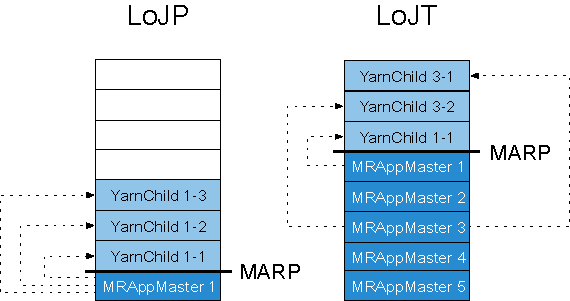
\includegraphics{./resources/marpValue.pdf}
    \caption[LoJP und LoJT in Hadoop]
    {LoJP und LoJT in Hadoop (entnommen aus \cite{Zhang2016}).
        Während beim LoJP sehr viel Speicher für Anwendungs"=Container ungenutzt bleibt, können beim LoJT nicht genügend Anwendungs"=Container allokiert werden, um die Anwendungen auszuführen.}
    \label{fig:marpValue}
\end{figure}

Damit bestimmt der \gls{MARP}"=Wert indirekt auch die maximale Anzahl an Anwendungen, die gleichzeitig ausgeführt werden können.
Da der \gls{MARP}"=Wert jedoch nicht während der Laufzeit dynamisch angepasst werden kann, haben \citeauthor{Zhang2016} in \cite{Zhang2016} einen Ansatz zur dynamischen Anpassung des \gls{MARP}"=Wertes zur Laufzeit von Hadoop vorgestellt.
Die entwickelte Selfbalancing"=Komponente passt den \gls{MARP}"=Wert abhängig von der Speicherauslastung der ausgeführten Anwendungen dynamisch zur Laufzeit an.
So wird der \gls{MARP}"=Wert, und damit auch die Anzahl der ausführbaren \gls{AppMstr}, verringert, wenn die Speicherauslastung sehr hoch ist, und erhöht, wenn die Speicherauslastung sehr niedrig ist.
Die Selfbalancing"=Komponente ermöglicht daher, dass immer die maximal mögliche Anzahl an Anwendungen ausgeführt werden kann.
Die Evaluation von \citeauthor{Zhang2016} ergab zudem, dass Anwendungen dadurch im Schnitt um bis zu 40 Prozent schneller ausgeführt werden können.
Zudem kann die dynamische Anpassung auch effizienter sein, als eine manuelle, statische Optimierung \cite{Zhang2016}.

\subsection{Analyse der Selfbalancing"=Komponente}
\label{subsec:selfbalancingAnalysis}

Da in dieser Fallstudie auch Mutationstests eingesetzt werden, bei denen die Selfbalancing"=Komponente entsprechend verändert wird (Implementierung in \cref{sec:implMutationTests}), wurde die Komponente zunächst analyisiert.
Sie besteht aus folgenden vier Java"=Klassen, welche den Kern der Komponente darstellen, und drei Shell"=Scripten, die als Verbindung zum Hadoop"=Cluster dienen:

\begin{itemize}
    \item Java"=Klassen:
    \begin{itemize}
        \item \texttt{controller.Controller}
        \item \texttt{effectuator.Effectuator}
        \item \texttt{monitor.ControlNodeMonitor}
        \item \texttt{monitor.MemUtilization}
    \end{itemize}
    \item Shell"=Scripte:
    \begin{itemize}
        \item \texttt{selfTuning-CapacityScheduler.sh}
        \item \texttt{selfTuning-controlNode.sh}
        \item \texttt{selfTuning-mem-controlNode.sh}
    \end{itemize}
\end{itemize}

Um den Zustand von Hadoop korrekt zu ermitteln, wird ein Kalman"=Filter in Form der Open"=Source"=Bibliotek JKalman\footnote{\url{https://jkalman.sourceforge.io/}} genutzt.
Der Kalman"=Filter wurde von \citeauthor{Kalman1960} erstmals in \cite{Kalman1960} beschrieben und wird genutzt, um \enquote{aus verrauschten und teils redundanten Messungen die Zustände und Parameter des Systems zu schätzen} \cite{Marchthaler2017}.
Der Filter lässt sich aufgrund seines Aufbaus zudem auch für Echtzeitanwendungen nutzen \cite{Marchthaler2017}.
Als einfaches Anwendungsbeispiel hierfür ist in \cite{Marchthaler2017} die Apollo"=Mondlandefähre genannt, \citeauthor{Strukov2001} nutzte ihn in \cite{Strukov2001} aber auch zur Reduktion der Komplexität im Controlling.
Für weitere Informationen zum Kalman"=Filter wie seinen Aufbau, Funktionsweise und Anwendung sei hier auf entsprechende Fachliteratur wie \zB \cite{Kim2016,Simon2006,Aggoun2004} verwiesen.

Die drei Shell-Scripte der Selfbalacing"=Komponente dienen zur Interaktion zwischen der Komponente und dem Cluster.
Die beiden zuletzt genannten Scripte werden von den beiden Monitor"=Klassen sekündlich gestartet und ermitteln basierend auf den Logs von Hadoop die Auslastung des Clusters.
Mithilfe von \texttt{selfTuning-controlNode.sh}, das von \texttt{ControlNodeMonitor} gestartet wird, wird die Anzahl an aktiven und wartenden YARN"=Jobs ermittelt und anschließend in der \texttt{controlNodeLog}"=Datei gespeichert.
Durch die Ausführung von \texttt{selfTuning-mem-controlNode.sh} (gestartet durch \texttt{MemUtilization}) wird dagegen die Auslastung des Speichers des Clusters ermittelt und in der \texttt{memLog}"=Datei notiert.

Die in den beiden Dateien enthaltenen Werten werden im Anschluss wiederum sekündlich vom \texttt{Controller} der Selfbalancing"=Komponente ausgelesen und mithilfe des Kalman"=Filters bereinigt.
Anschließend werden die Algorithmen \cite{Zhang2016} zum Berechnen des neuen \gls{MARP}"=Wertes ausgeführt.

Um den dadurch neu ermittelten \gls{MARP}"=Wert anzuwenden, wird abschließend mithilfe des \texttt{Effectuator}s das dritte Shell"=Script \texttt{selfTuning-CapacityScheduler.sh} ausgeführt.
Mithilfe dieses Shell"=Scriptes wird der neue MARP"=Wert in der Konfiguration des \emph{Capacity Schedulers} gespeichert.


\section{Plattform Hadoop"=Benchmark}
\label{sec:hadoopBenchmark}

\citeauthor{Zhang2016} haben im Rahmen ihrer gesamten Forschungsarbeit an der Selfbalancing"=Komponente darüber hinaus auch die Open"=Source"=Plattform Hadoop"=Benchmark entwickelt\footnote{\url{https://github.com/Spirals-Team/hadoop-benchmark}}.
Sie dient zur einfachen und schnellen Ausführung eines Hadoop"=Clusters und wurde speziell zum Einsatz in der Forschung erstellt.
Dadurch kann sie auch mit geringem Aufwand an eigene Bedürfnisse angepasst werden.

Zur Ausführung des Clusters wird die Virtualisierungs"=Software Docker\footnote{\url{https://www.docker.com/}} und das dazugehörige \emph{Docker Machine} genutzt.
Durch die Virtualisierung wird für jeden Hadoop"=Node eine Docker"=Machine gestartet, auf der der Hadoop"=Node wiederum in einem Docker"=Container ausgeführt wird.
Verbunden werden die Nodes dabei mithilfe eines \emph{Docker" Swarm}s\footnote{\url{https://docs.docker.com/engine/swarm/}}.

\begin{figure}[h]
    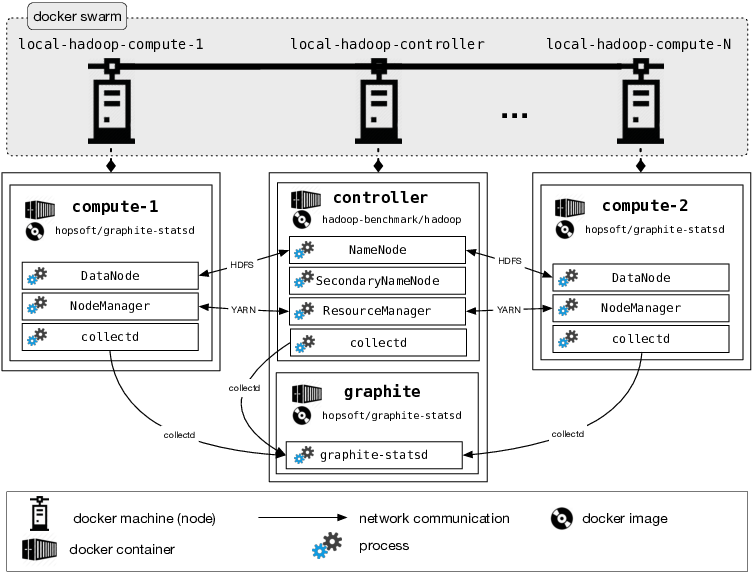
\includegraphics{./resources/hadoopBenchmarkArch.png}
    \caption[High"=Level"=Architektur von Hadoop"=Benchmark]
    {High"=Level"=Architektur von Hadoop"=Benchmark (entnommen aus \cite{abb:hadoopBenchmarkArch})}
    \label{fig:hadoopBenchmarkArchitecture}
\end{figure}

Docker"=Machine ist keine komplette Virtualisierungs"=Software, sondern nutzt hier VirtualBox\footnote{\url{https://www.virtualbox.org/}}, um virtuelle Maschinen zu starten, die mit dem Betriebssystem \emph{Boot2Docker} ausgestattet sind.
Boot2Docker ist eine leichtgewichtige Linux"=Distribution, auf der Docker bereits vorinstalliert ist \cite{DockerMachineGettingStartedVm}.

Mit \emph{Graphite}\footnote{\url{https://graphiteapp.org/}} ist zudem ein Monitoring"=Tool enthalten, mit dem die Systemwerte wie CPU- oder Speicher"=Auslastung des Clusters überwacht und analysiert werden kann.
Jeder Hadoop"=Container enthält dazu das Tool \emph{collectd}\footnote{\url{https://collectd.org/}}, was das Monitoring des Containers auf Systemebene übernimmt und die Daten an den Graphite"=Container übermittelt.

Da mithilfe der Plattform auch unterschiedliche Hadoop"=Konfigurationen ausgeführt werden können, ist die Plattform in mehrere Szenarien unterteilt.
Jedes Szenario stellt eine Hadoop"=Konfiguration dar, die vollständig angepasst werden kann.
Jedes Szenario enthält daher eine \emph{Dockerfile}, aus der die Docker"=Images und -Container erstellt werden, weitere für Hadoop benötigte Daten und Einstellungen, sowie dazugehörige generelle Einstellungen des Szenarios.
Die Plattform enthält bereits mehrere Szenarien, \uA Hadoop in der Version 2.7.1 ohne Anpassungen sowie ein darauf basierendes Szenario mit der Selfbalancing"=Komponente.
Aufgrund eines der Kernkonzepte von Docker, wonach Docker"=Images auf einem passenden, bereits vorhandenen Images aufbauen können bzw. sollten \cite{DockerdevBestPractice}, ist es möglich, neue Szenarien basierend auf bereits vorhandenen zu entwickeln.

Zum Starten des Clusters ist ein Script enthalten, welches basierend auf dem zu nutzenden Szenario das Cluster in der entsprechenden Konfiguration startet.

In der Plattform Hadoop"=Benchmark sind auch bereit einige Benchmarks integriert:

\begin{itemize}
    \item Hadoop Mapreduce Examples
    \item Intel HiBench\footnote{\url{https://github.com/intel-hadoop/HiBench}}
    \item \gls{SWIM} \footnote{\url{https://github.com/SWIMProjectUCB/SWIM}}
\end{itemize}

Die Benchmarks werden ebenfalls mithilfe der in der Plattform enthaltenen Scripte gestartet.
Hierbei besitzt jeder Benchmark ein eigenes Start"=Script, das den Benchmark in einem Docker"=Container startet und die entsprechende \gls{Anwendung} so dem Cluster zur Ausführung übergibt.
Die Ausführung einer \gls{Anwendung} mithilfe des entsprechenden Start"=Scriptes sowie das Beenden einer \gls{Anwendung} ist in \cref{app:hadoopCmds} beispielhaft aufgezeigt.

Genauere Informationen zu den in der Plattform enthaltenen Benchmarks sind in \cref{sec:appOverview} erläutert.

